\documentclass[11pt,a4paper]{article}
\usepackage[margin=1in]{geometry}
\usepackage[T1]{fontenc}
\usepackage[utf8]{inputenc}
\usepackage{graphicx}
\usepackage{booktabs}
\usepackage{float}
\usepackage{tabularx}
\usepackage{array}
\usepackage{hyperref}
\usepackage{xcolor}
\hypersetup{colorlinks=true,linkcolor=blue,urlcolor=blue}

\title{SEM Dendrite Segmentation: Comparative Technical Report}
\author{Automated Report Generator}
\date{\today}

\begin{document}
\maketitle

\section*{Abstract}
This report summarizes pixel-level semantic segmentation of lithium dendrites in SEM images using two pipelines:
(1) a deterministic classic morphology pipeline and
(2) a YOLO segmentation model.
The evaluation set includes 13 labeled images.
Average Dice scores are Classic=0.908 and YOLO=0.478.
The report includes quantitative metrics, method comparison tables, and visual success/failure analysis.

\section*{Methodology}
\textbf{Classic Pipeline:} pre-processing (normalization, CLAHE, bilateral denoising), threshold-based segmentation,
morphological cleaning/reconstruction, branch separation, and skeleton extraction.\\
\textbf{Deep Learning Pipeline:} transfer-learned YOLO segmentation model with binary mask output per image.\\
\textbf{Evaluation Metrics:} Dice, IoU, Precision, Recall measured against manual ground-truth masks.

\section*{Results and Discussion}
\subsection*{Average Metrics}
\begin{table}[H]
\centering
\begin{tabular}{lcccc}
\toprule
Method & Dice & IoU & Precision & Recall \\
\midrule
Classic & 0.908 & 0.847 & 0.847 & 1.000 \\
YOLO & 0.478 & 0.323 & 0.358 & 0.748 \\
\bottomrule
\end{tabular}
\caption{Average segmentation metrics across available predictions.}
\end{table}

\subsection*{Per-Image Comparison}
\begin{table}[H]
\centering
\scriptsize
\begin{tabular}{lcccccccc}
\toprule
Image & C-Dice & C-IoU & C-Prec & C-Rec & Y-Dice & Y-IoU & Y-Prec & Y-Rec \\
\midrule
2e-9\_100s\_002 & 0.923 & 0.857 & 0.857 & 1.000 & 0.579 & 0.407 & 0.409 & 0.991 \\

2e-9\_100s\_014 & 0.931 & 0.872 & 0.872 & 1.000 & 0.655 & 0.487 & 0.560 & 0.789 \\

2e-9\_100s\_017 & 0.699 & 0.538 & 0.538 & 1.000 & 0.103 & 0.055 & 0.066 & 0.241 \\

2e-9\_100s\_019 & 0.997 & 0.995 & 0.995 & 1.000 & 0.596 & 0.424 & 0.454 & 0.865 \\

70nm\_diameter\_100nm\_pitch\_008 & 0.927 & 0.863 & 0.863 & 1.000 & 0.438 & 0.280 & 0.302 & 0.798 \\

70nm\_diameter\_100nm\_pitch\_012 & 0.919 & 0.850 & 0.850 & 1.000 & 0.523 & 0.354 & 0.399 & 0.758 \\

70nm\_diameter\_100nm\_pitch\_022 & 0.995 & 0.991 & 0.991 & 1.000 & 0.454 & 0.293 & 0.374 & 0.577 \\

70nm\_diameter\_100nm\_pitch\_031 & 1.000 & 1.000 & 1.000 & 1.000 & 0.359 & 0.218 & 0.272 & 0.527 \\

Ag\_1e-8\_008 & 1.000 & 1.000 & 1.000 & 1.000 & 0.436 & 0.278 & 0.325 & 0.660 \\

Ag\_1e-9\_\_02\_016 & 0.906 & 0.828 & 0.828 & 1.000 & 0.560 & 0.389 & 0.432 & 0.796 \\

Ag\_2e-9\_013 & 0.760 & 0.612 & 0.612 & 1.000 & 0.518 & 0.350 & 0.351 & 0.994 \\

Ag\_2e-9\_014 & 0.753 & 0.603 & 0.603 & 1.000 & 0.479 & 0.315 & 0.316 & 0.994 \\

Ag\_40nm\_pitch\_014 & 1.000 & 1.000 & 1.000 & 1.000 & 0.514 & 0.346 & 0.395 & 0.736 \\
\bottomrule
\end{tabular}
\caption{Per-image metric comparison (first 13 rows). Full table is exported to CSV.}
\end{table}

\subsection*{Failure Analysis}
Number of failures under Dice threshold: 6.
\begin{table}[H]
\centering
\scriptsize
\begin{tabularx}{\linewidth}{llcccX}
\toprule
Image & Method & Dice & Precision & Recall & Estimated Cause \\
\midrule
2e-9\_100s\_017 & YOLO & 0.103 & 0.066 & 0.241 & Fundamental mismatch - wrong region or severe artifacts (Classic succeeds -> likely OOD sample for YOLO) \\

70nm\_diameter\_100nm\_pitch\_031 & YOLO & 0.359 & 0.272 & 0.527 & Fundamental mismatch - wrong region or severe artifacts (Classic succeeds -> likely OOD sample for YOLO) \\

Ag\_1e-8\_008 & YOLO & 0.436 & 0.325 & 0.660 & Over-segmentation - noise included as dendrite (Classic succeeds -> likely OOD sample for YOLO) \\

70nm\_diameter\_100nm\_pitch\_008 & YOLO & 0.438 & 0.302 & 0.798 & Over-segmentation - noise included as dendrite (Classic succeeds -> likely OOD sample for YOLO) \\

70nm\_diameter\_100nm\_pitch\_022 & YOLO & 0.454 & 0.374 & 0.577 & Fundamental mismatch - wrong region or severe artifacts (Classic succeeds -> likely OOD sample for YOLO) \\

Ag\_2e-9\_014 & YOLO & 0.479 & 0.316 & 0.994 & Over-segmentation - noise included as dendrite (Classic succeeds -> likely OOD sample for YOLO) \\
\bottomrule
\end{tabularx}
\caption{Failure characterization based on precision/recall patterns.}
\end{table}

\subsection*{Visual Analysis (Successes and Failures)}
\begin{figure}[H]
\centering
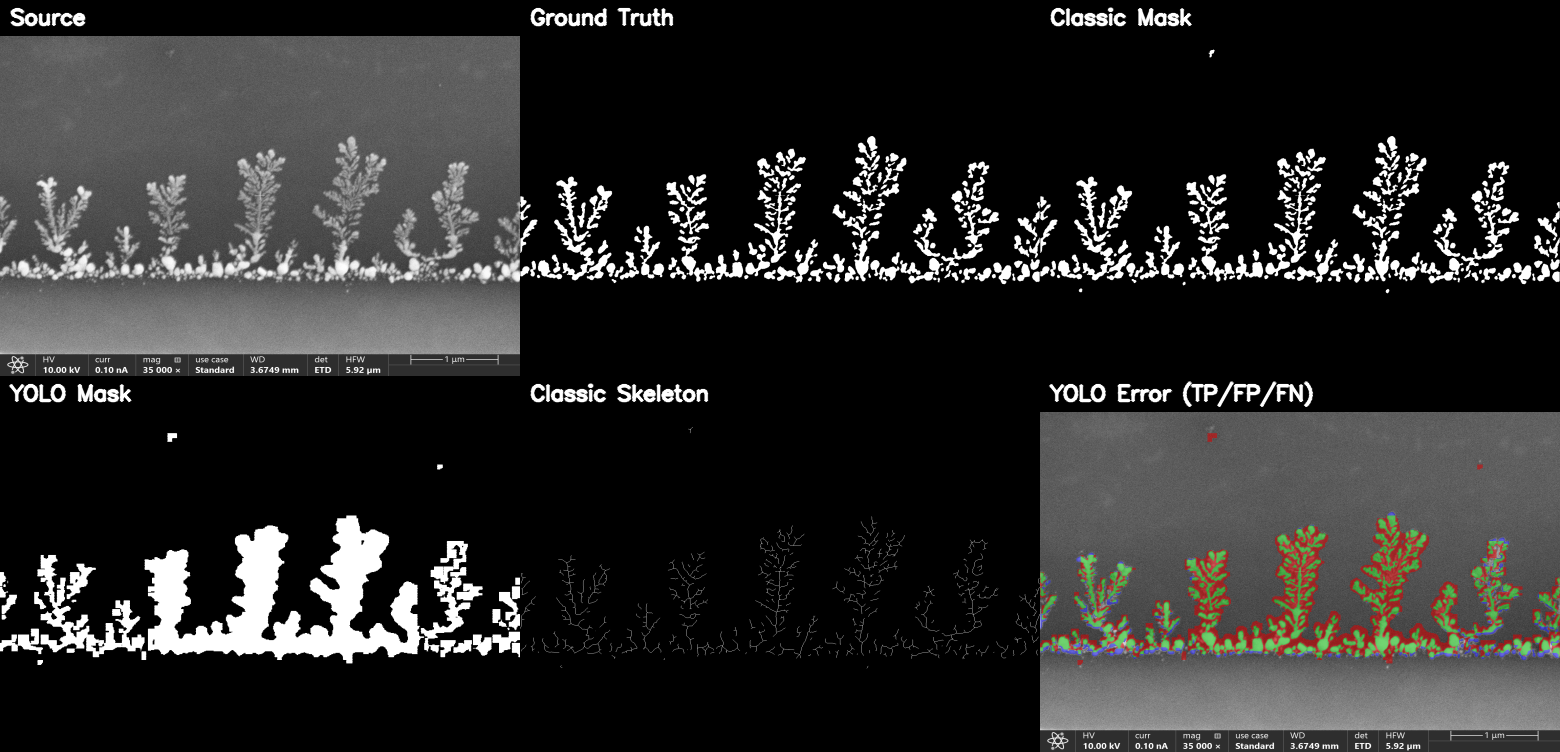
\includegraphics[width=0.96\linewidth]{assets/cases/2e-9_100s_019_analysis.png}
\caption{Success case: 2e-9\_100s\_019 (combined Dice=0.797)}
\end{figure}

\begin{figure}[H]
\centering
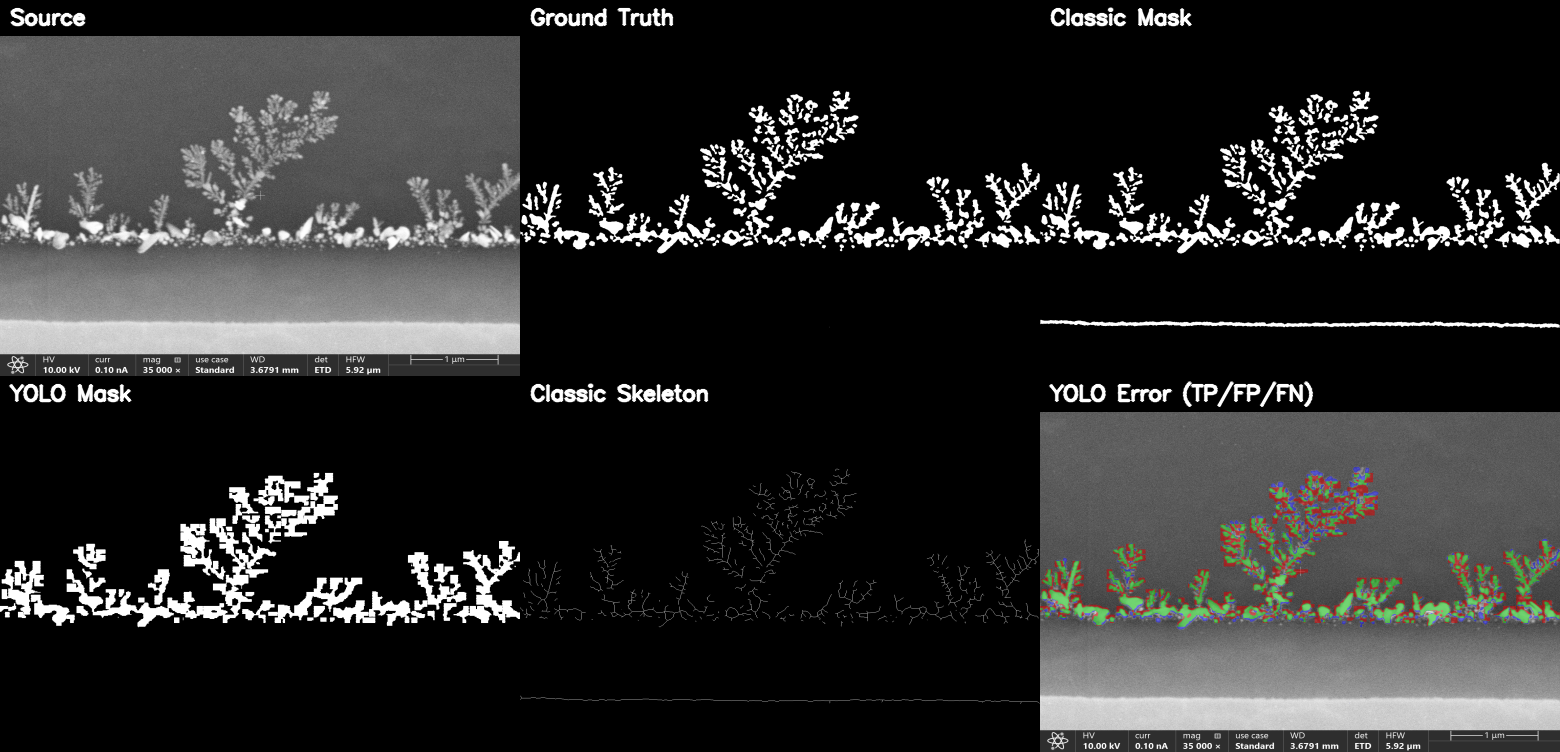
\includegraphics[width=0.96\linewidth]{assets/cases/2e-9_100s_014_analysis.png}
\caption{Success case: 2e-9\_100s\_014 (combined Dice=0.793)}
\end{figure}

\begin{figure}[H]
\centering
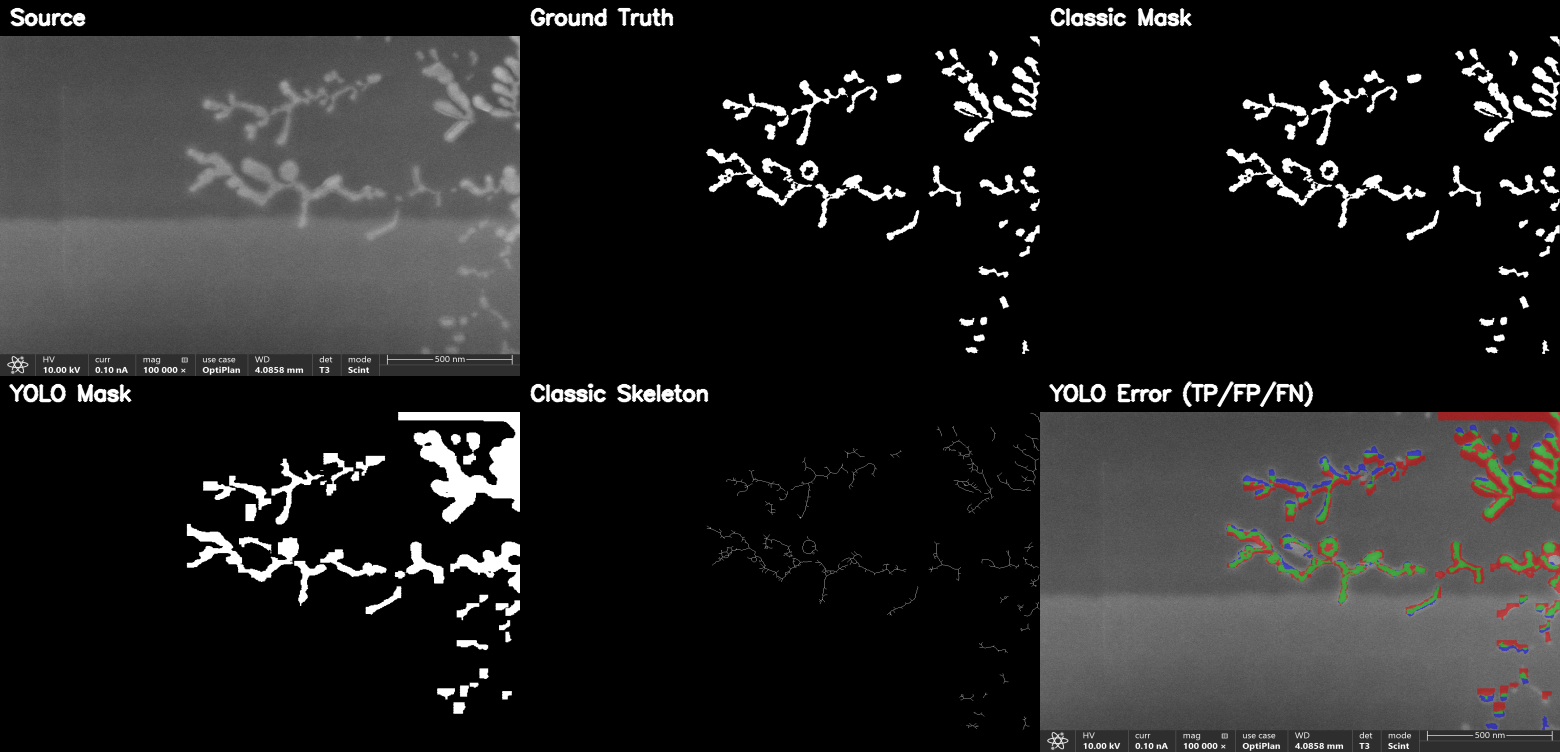
\includegraphics[width=0.96\linewidth]{assets/cases/Ag_40nm_pitch_014_analysis.png}
\caption{Success case: Ag\_40nm\_pitch\_014 (combined Dice=0.757)}
\end{figure}

\begin{figure}[H]
\centering
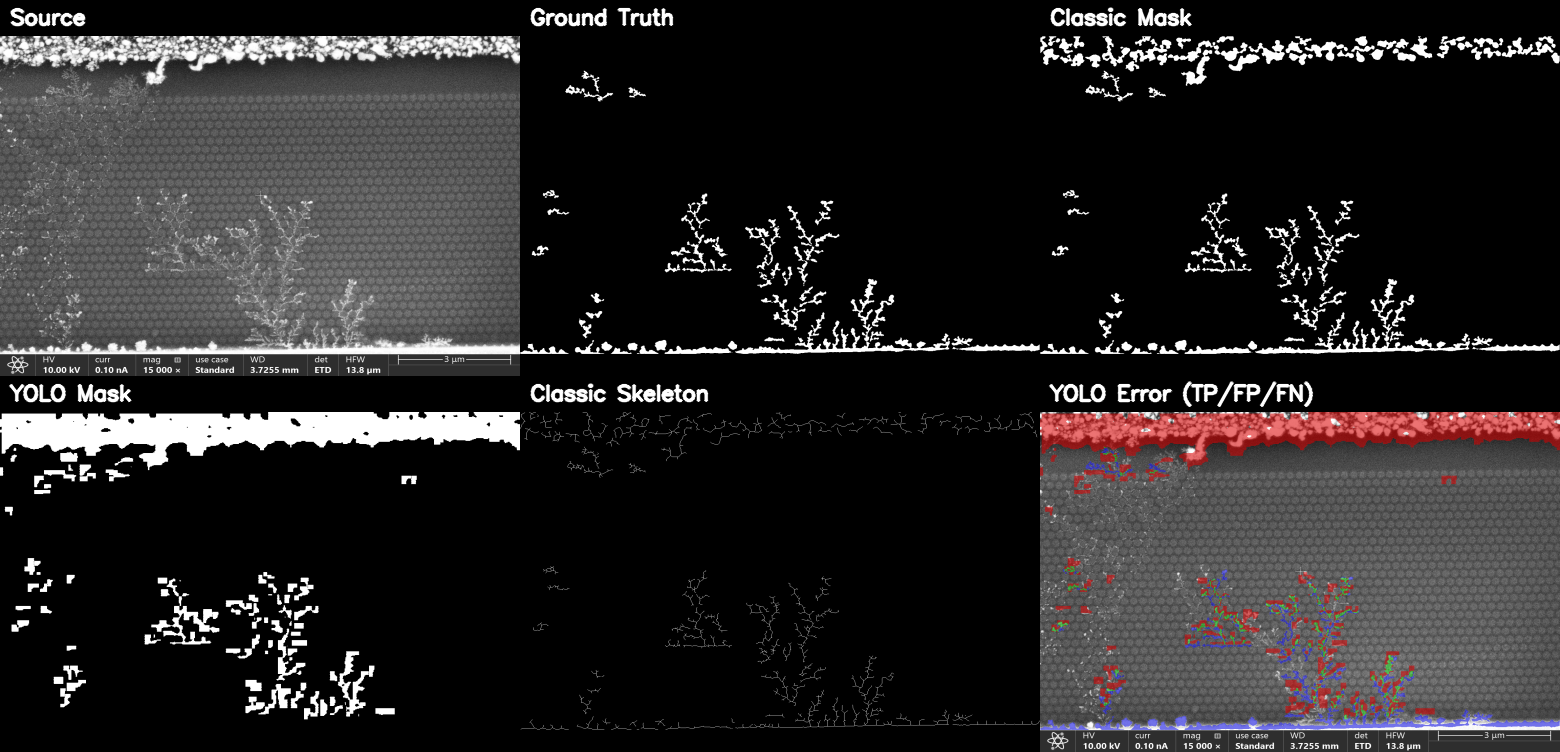
\includegraphics[width=0.96\linewidth]{assets/cases/2e-9_100s_017_analysis.png}
\caption{Failure case: 2e-9\_100s\_017 (combined Dice=0.401)}
\end{figure}

\begin{figure}[H]
\centering
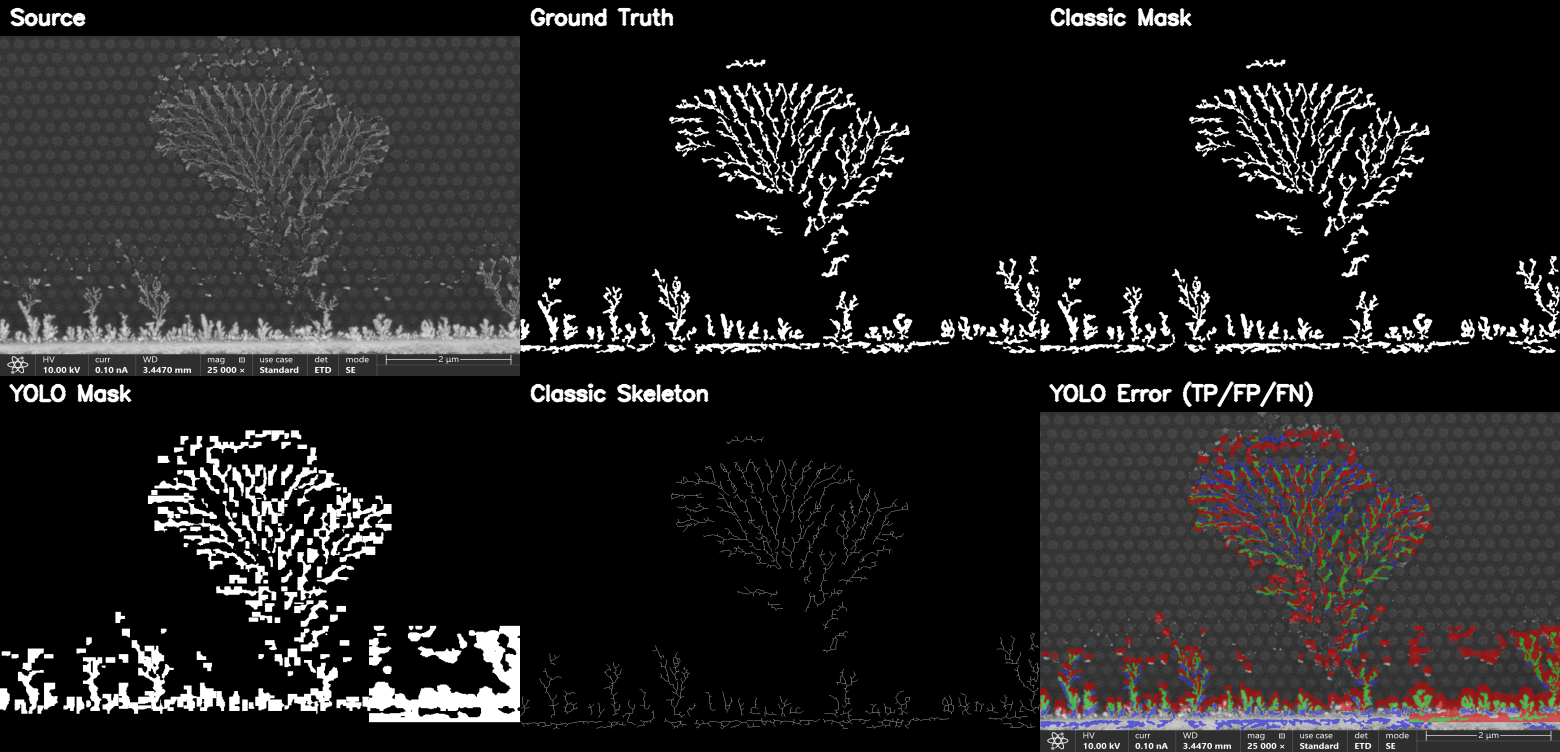
\includegraphics[width=0.96\linewidth]{assets/cases/70nm_diameter_100nm_pitch_031_analysis.png}
\caption{Failure case: 70nm\_diameter\_100nm\_pitch\_031 (combined Dice=0.679)}
\end{figure}

\begin{figure}[H]
\centering
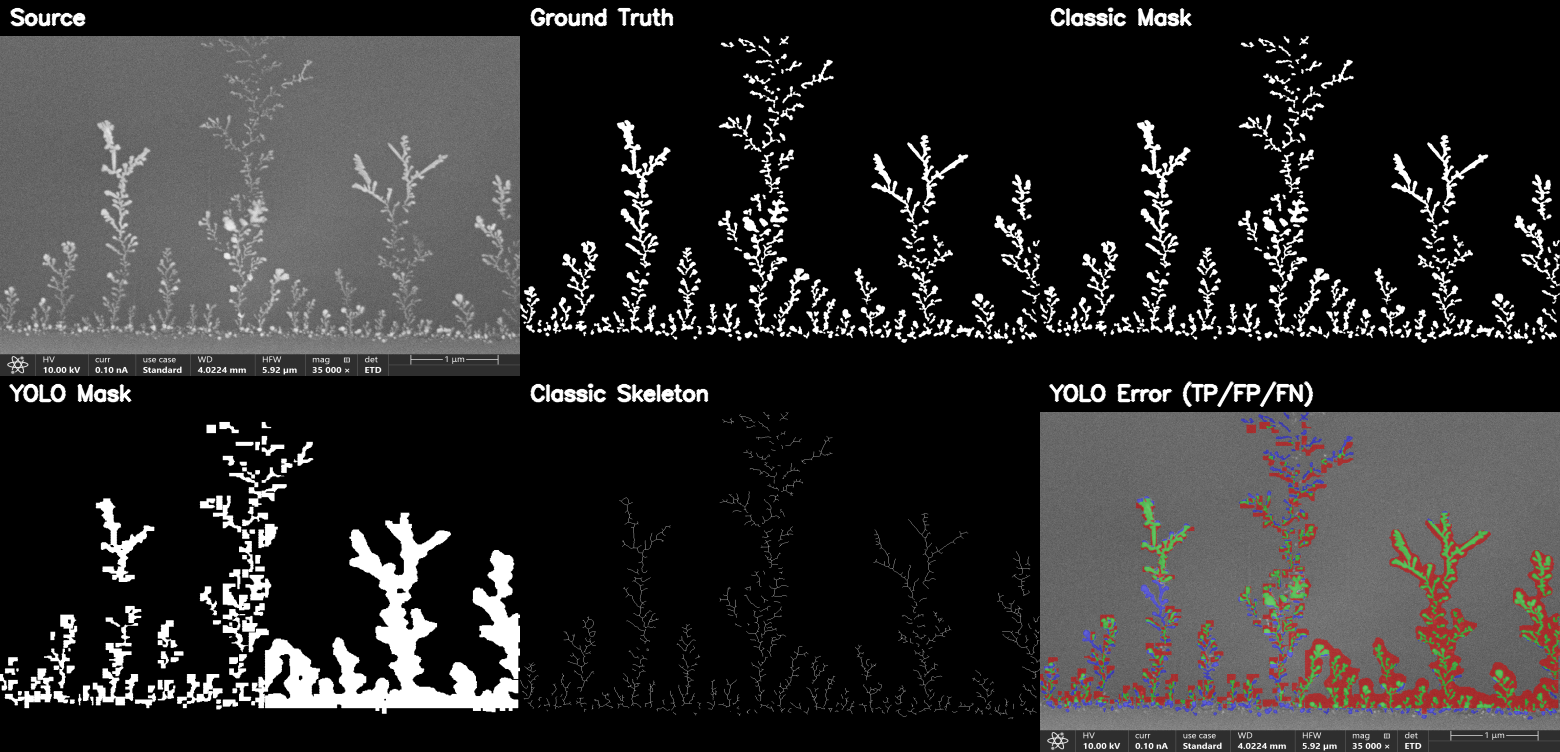
\includegraphics[width=0.96\linewidth]{assets/cases/Ag_1e-8_008_analysis.png}
\caption{Failure case: Ag\_1e-8\_008 (combined Dice=0.718)}
\end{figure}

\subsection*{YOLO Training Diagnostics}
\begin{figure}[H]
\centering
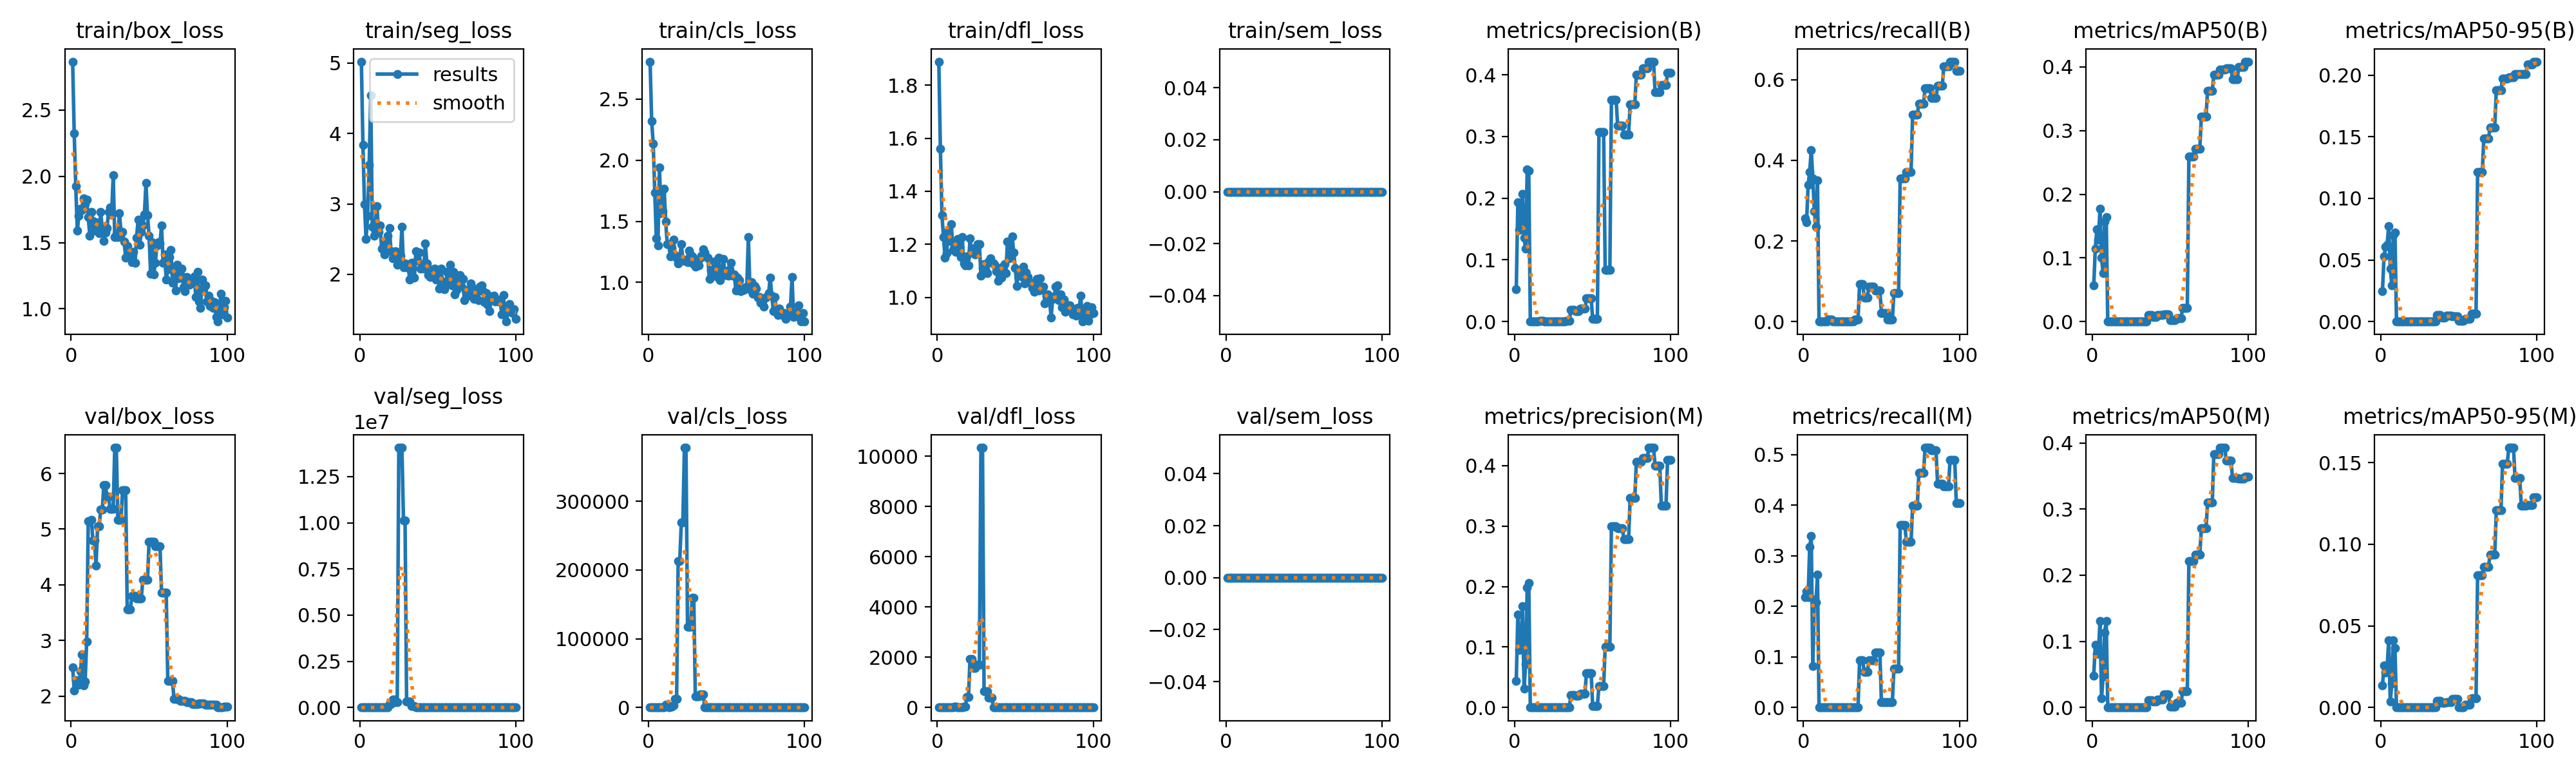
\includegraphics[width=0.92\linewidth]{assets/training/results.png}
\caption{YOLO training metrics over epochs}
\end{figure}

\begin{figure}[H]
\centering
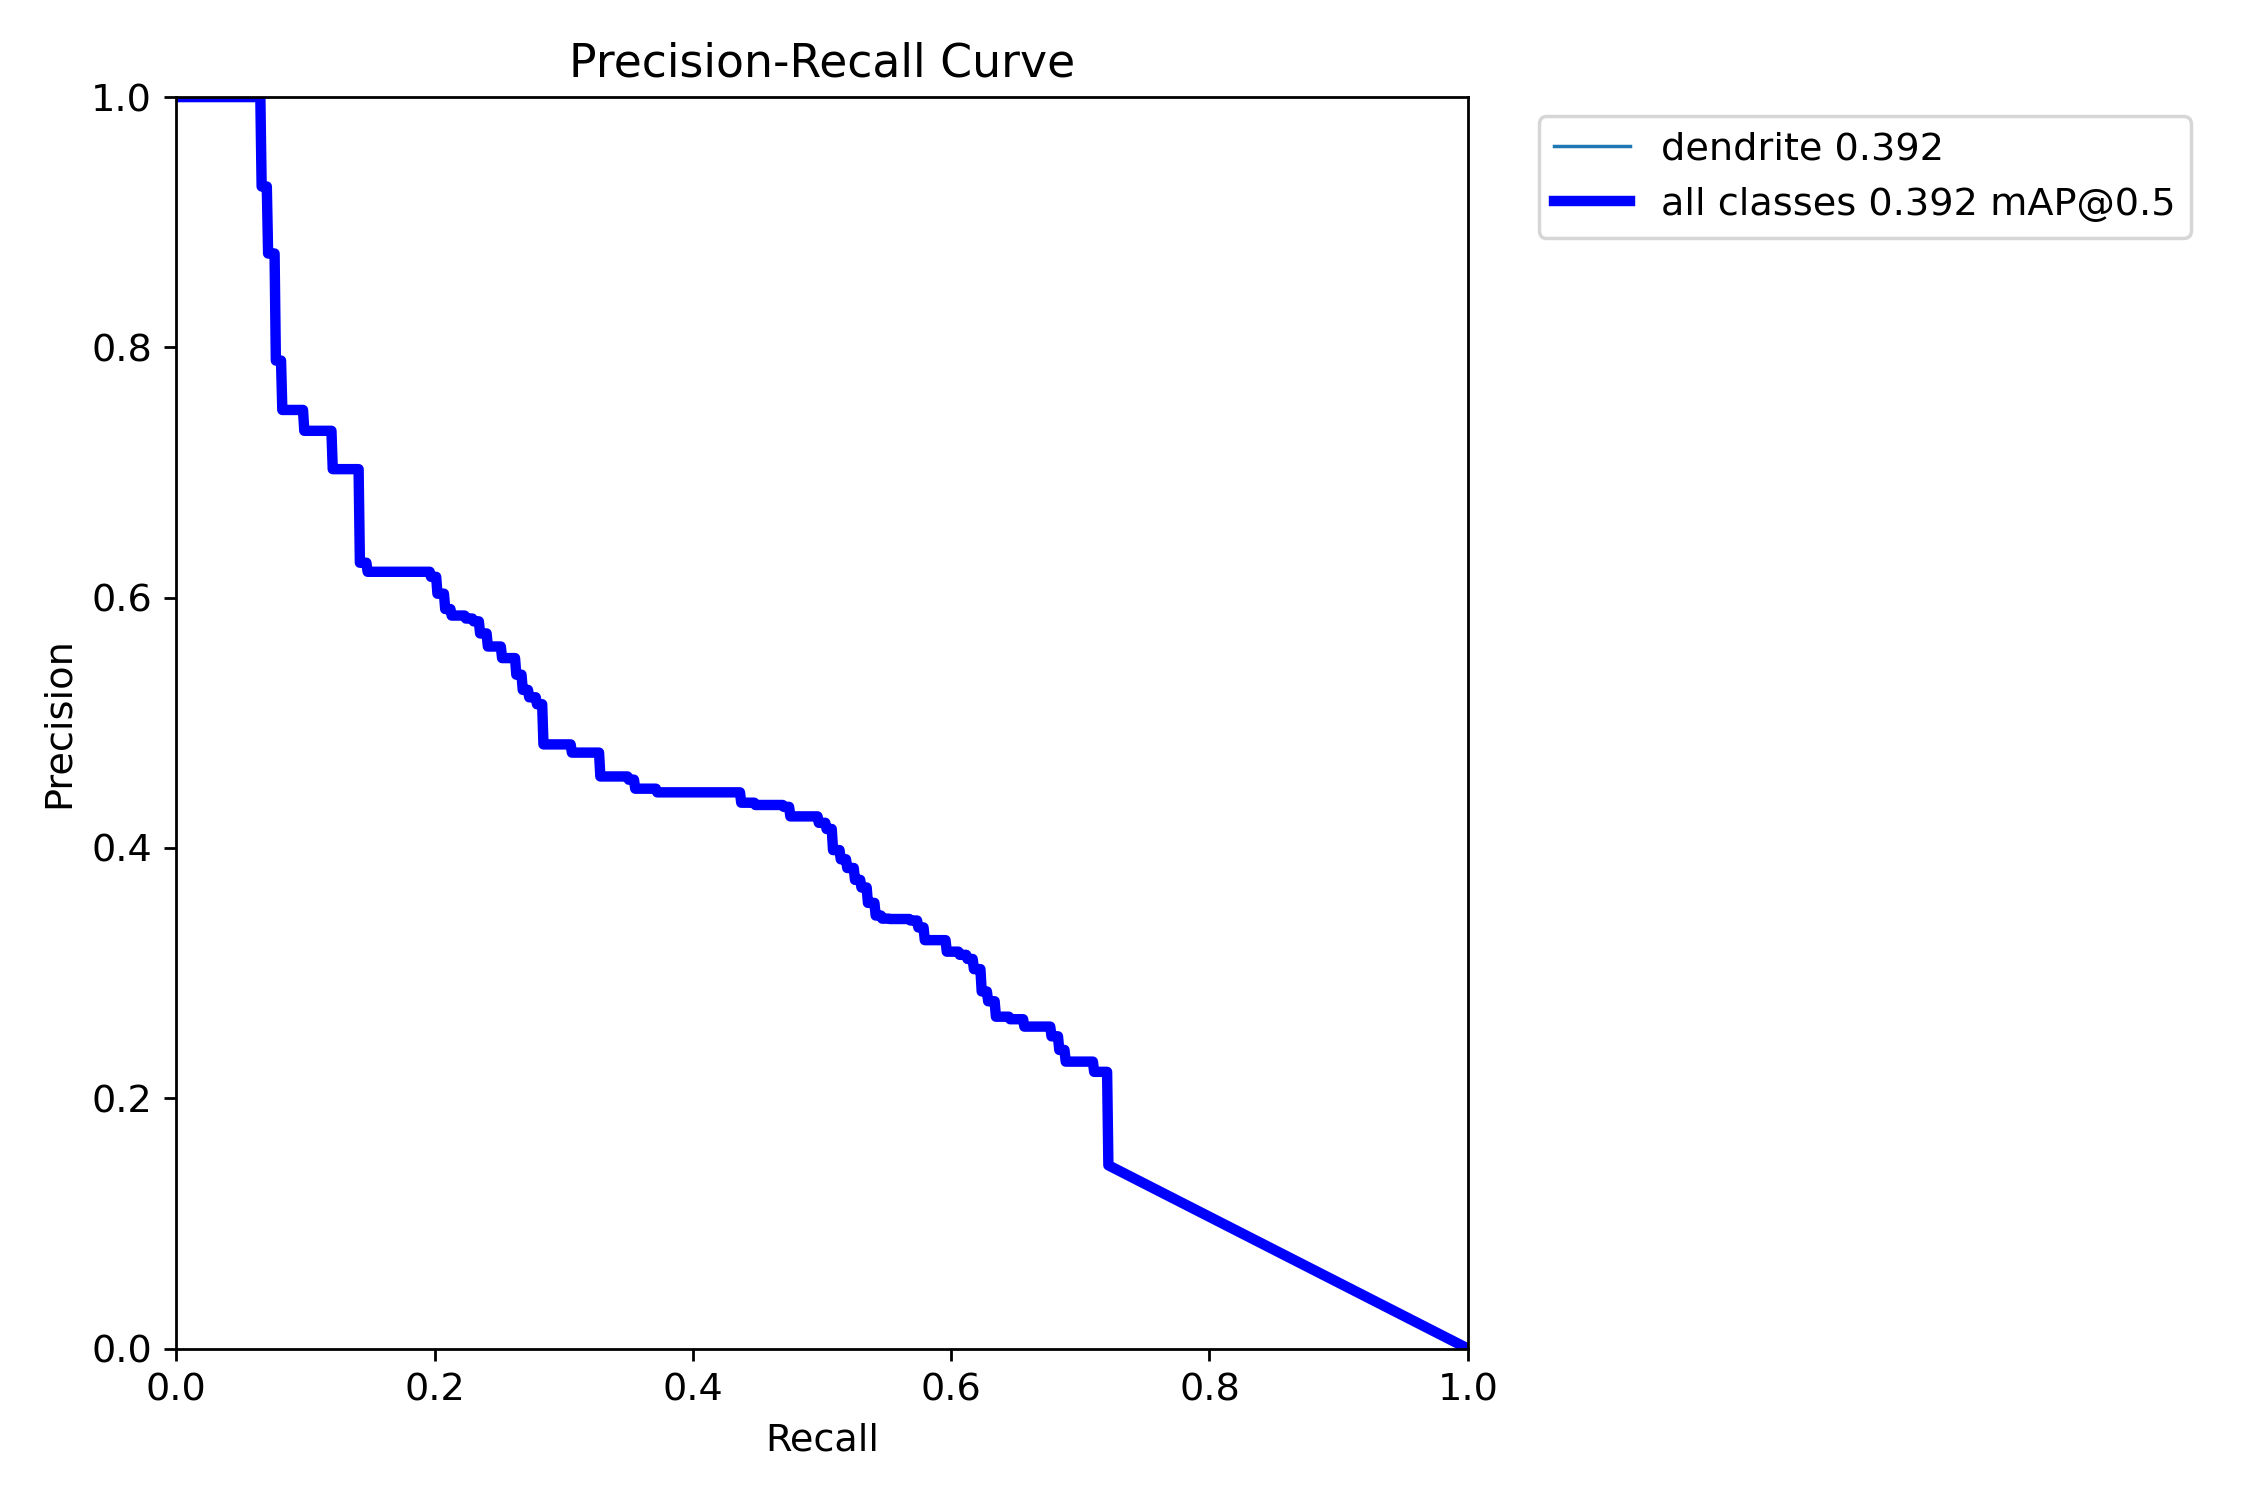
\includegraphics[width=0.92\linewidth]{assets/training/MaskPR_curve.png}
\caption{Mask precision-recall curve}
\end{figure}

\begin{figure}[H]
\centering
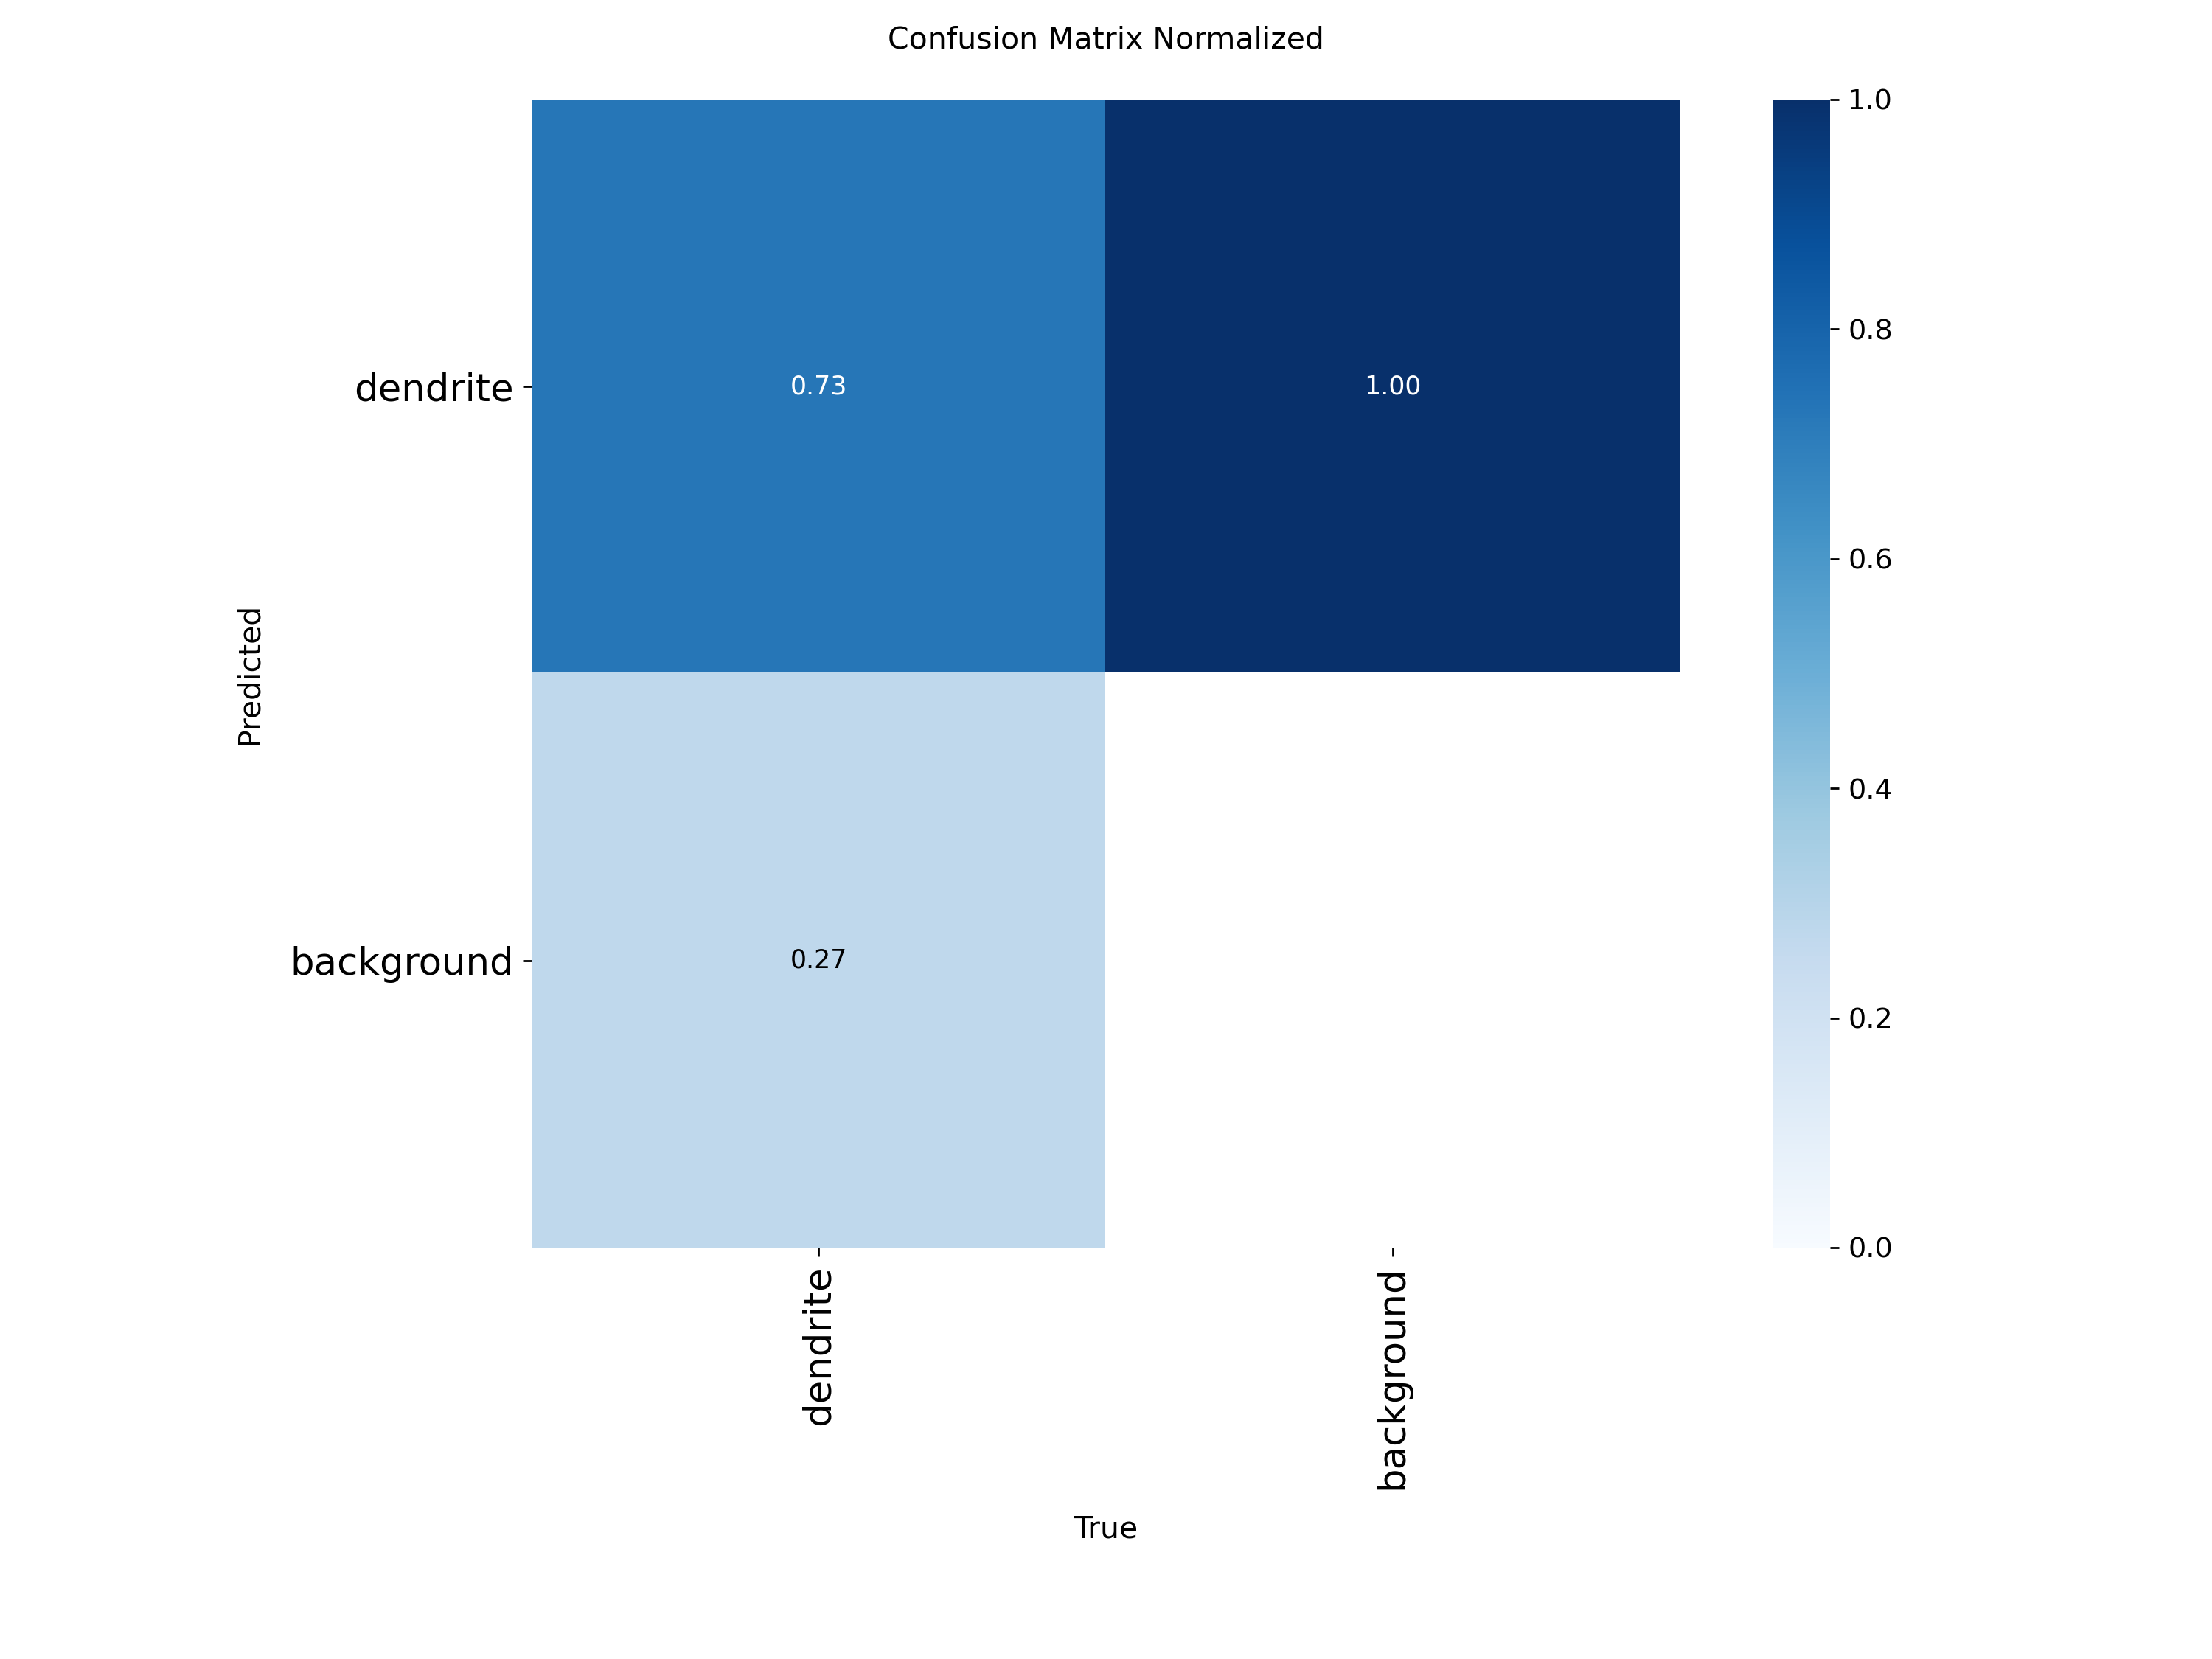
\includegraphics[width=0.92\linewidth]{assets/training/confusion_matrix_normalized.png}
\caption{Normalized confusion matrix}
\end{figure}

\section*{Conclusions}
The generated artifacts support the project submission requirements:
technical report format, quantitative metrics, comparison tables, and qualitative visual analysis.
Use this report as a reproducible baseline and regenerate it whenever new experiments are produced.

\end{document}
